\title{Casper the Friendly Finality Gadget: Basic Structure}
\author{
        Vitalik Buterin \\
        Ethereum Foundation
}
\date{\today}

\documentclass[12pt]{article}
\usepackage{graphicx}
\usepackage{tabularx}
\newtheorem{definition}{Definition}

\begin{document}
\maketitle
\begin{abstract}
We give an introduction to the consensus algorithm details of Casper: the Friendly Finality Gadget, as an overlay on an existing proof of work blockchain such as Ethereum. Byzantine fault tolerance analysis is included, but economic incentive analysis is out of scope.
\end{abstract}

\section{Principles}
Casper the Friendly Finality Gadget is designed as an overlay that must be built on top of some kind of ``proposal mechanism'' - a mechanism which ``proposes'' blocks which the Casper mechanism can then set in stone by ``finalizing'' them. The Casper mechanism depends on the proposal mechanism for liveness, but not safety; that is, if the proposal mechanism is entirely corrupted and controlled by adversaries, then the adversaries can prevent Casper from finalizing any blocks, but cannot cause a safety failure in Casper; that is, they cannot force Casper to finalize two conflicting blocks.

The base mechanism is heavily inspired by partially synchronous systems such as Tendermine [cite] and PBFT [cite], and thus has $\frac{1}{3}$ Byzantine fault tolerance and is safe under asynchrony and dependent on the proposal mechanism for liveness. We later introduce a modification which increases Byzantine fault tolerance to $\frac{1}{2}$, with the proviso that attackers with size $\frac{1}{3} < x < \frac{1}{2}$ can delay new blocks being finalized by some period of time $D$ (think $D \approx$ 3 weeks), at the cost of a ``tradeoff synchrony assumption'' where fault tolerance decreases as network latency goes up, decreasing to potentially zero when network latency reaches $D$.

In the Casper Phase 1 implementation for Ethereum, the ``proposal mechanism'' is the existing proof of work chain, modified to have a greatly reduced block reward because the chain no longer relies as heavily on proof of work for security, and we describe how the Casper mechanism, and fork choice rule, can be ``overlaid'' onto the proof of work mechanism in order to add Casper's guarantees.

\section{Introduction, Protocol I}

In the Casper protocol, there exists a set of validators, and in each \textit{epoch} (see below) validators have the ability to send two kinds of messages: $$[PREPARE, epoch, hash, epoch_{source}, hash_{source}]$$ and $$[COMMIT, epoch, hash]$$

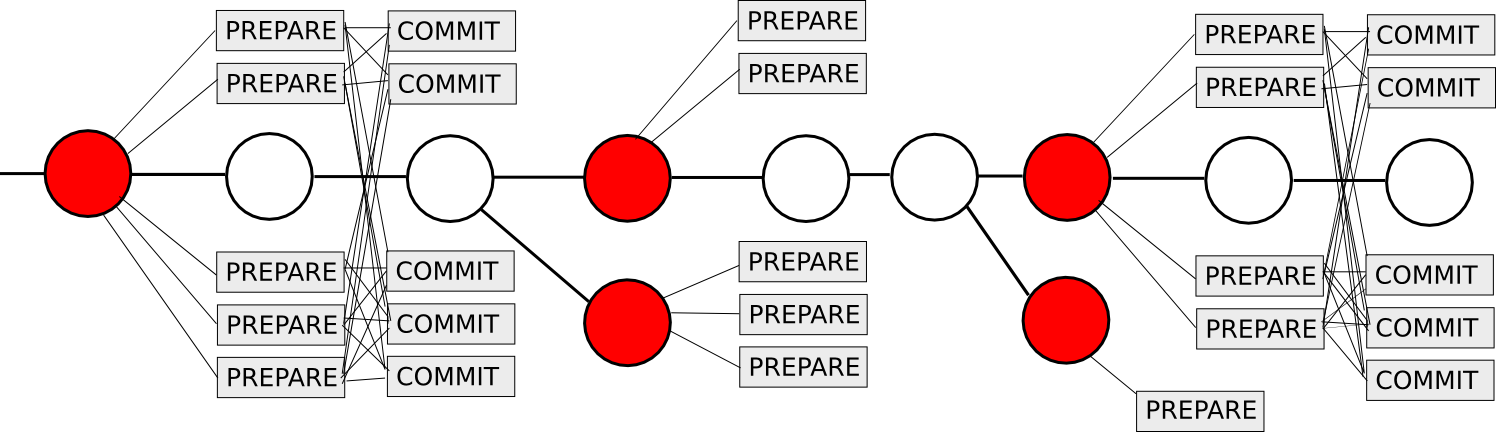
\includegraphics[width=400px]{prepares_commits.png}

An \textit{epoch} is a period of 100 blocks; epoch $n$ begins at block $n * 100$ and ends at block $n * 100 + 99$. A \textit{checkpoint for epoch $n$} is a block with number $n * 100 - 1$; in a smoothly running blockchain there will usually be only one checkpoint per epoch, but due to natural network latency or deliberate attacks there may be multiple competing checkpoints during some epochs. The \textit{parent checkpoint} of a checkpoint is the 100th ancestor of the checkpoint block, and an \textit{ancestor checkpoint} of a checkpoint is either the parent checkpoint, or an ancestor checkpoint of the parent checkpoint.

We define the \textit{ancestry hash} of a checkpoint as follows:

\begin{itemize}
\item The ancestry hash of the implied ``genesis checkpoint'' of epoch 0 is thirty two zero bytes.
\item The ancestry hash of any other checkpoint is the keccak256 hash of the ancestry hash of its parent checkpoint concatenated with the hash of the checkpoint.
\end{itemize}

Ancestry hashes thus form a direct hash chain, and otherwise have a one-to-one correspondence with checkpoint hashes.

During epoch $n$, validators are expected to send prepare and commit messages specifying $n$ as their $epoch$, and the ancestry hash of some checkpoint for epoch $n$ as their $hash$. Prepare messages are expected to specify as $hash_{source}$ a checkpoint for any previous epoch which is an ancestor of the $hash$, and which is \textit{justified} (see below), and the $epoch_{source}$ is expected to be the epoch of that checkpoint.

Each validator has a \textit{deposit size}; when a validator joins their deposit size is equal to the number of coins that they deposited, and from there on each validator's deposit size rises and falls as the validator receives rewards and penalties. For the rest of this paper, when we say ``$\frac{2}{3}$ of validators", we are referring to a \textit{deposit-weighted} fraction; that is, a set of validators whose combined deposit size equals to at least $\frac{2}{3}$ of the total deposit size of the entire set of validators. We also use ``$\frac{2}{3}$ commits" as shorthand for ``commits from $\frac{2}{3}$ of validators". At first, we will consider the set of validators, and their deposit sizes, static, but in later sections we will introduce the notion of validator set changes.

If, during an epoch $e$, for some specific ancestry hash $h$, for any specific ($epoch_{source}, hash_{source}$ pair), there exist $\frac{2}{3}$ prepares of the form $$[PREPARE, e, h, epoch_{source}, hash_{source}]$$, then $h$ is considered \textit{justified}. If $\frac{2}{3}$ commits are sent of the form $$[COMMIT, e, h]$$ then $h$ is considered \textit{finalized}.

We also add the following requirements:

\begin{itemize}
\item For a checkpoint to be finalized, it must be justified.
\item For a checkpoint to be justified, the $hash_{source}$ used to justify it must itself be justified.
\item Prepare and commit messages are only accepted as part of blocks; that is, for a client to see $\frac{2}{3}$ commits of some hash, they must receive a block such that in the chain terminating at that block $\frac{2}{3}$ commits for that hash have been included and processed.
\end{itemize}

This gives substantial gains in implementation simplicity, because it means that we can now have a fork choice rule where the ``score'' of a block only depends on the block and its children, putting it into a similar category as more traditional PoW-based fork choice rules such as the longest chain rule and GHOST. However, this fork choice rule is also \textit{finality-bearing}: there exists a ``finality'' mechanism that has the property that (i) the fork choice rule always prefers finalized blocks over non-finalized competing blocks, and (ii) it is impossible for two incompatible checkpoints to be finalized unless at least $\frac{1}{3}$ of the validators violated a \textit{slashing condition} (see below).

There are two slashing conditions:

\begin{enumerate}
\item \textbf{NO\_DBL\_PREPARE}: a validator cannot prepare two different checkpoints for the same epoch.
\item \textbf{PREPARE\_COMMIT\_CONSISTENCY}: if a validator has made a commit with epoch $n$, they cannot make a prepare with $epoch > n$ and $epoch_{source} < n$.
\end{enumerate}

Earlier versions of Casper had four slashing conditions, but we can reduce to two because of the three modifications above; they ensure that blocks will not register commits or prepares that violate the other two conditions.

\section{Proof Sketch of Safety and Plausible Liveness}

We give a proof sketch of two properties of this scheme: \textit{accountable safety} and \textit{plausible liveness}. Accountable safety means that two conflicting checkpoints cannot be finalized unless at least $\frac{1}{3}$ of validators violate a slashing condition. Honest validators will not violate slashing conditions, so this implies the usual Byzantine fault tolerance safety property, but expressing this in terms of slashing conditions means that we are actually proving a stronger claim: if two conflicting checkpoints get finalized, then at least $\frac{1}{3}$ of validators were malicious, \textit{and we know whom to blame, and so we can maximally penalize them in order to make such faults expensive}.

Plausible liveness means that it is always possible for $\frac{2}{3}$ of honest validators to finalize a new checkpoint, regardless of what previous events took place.

Suppose that two conflicting checkpoints $A$ (epoch $e_A$) and $B$ (epoch $e_B$) are finalized.

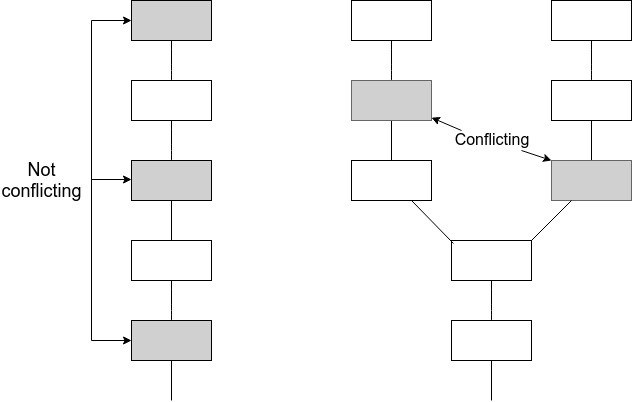
\includegraphics[width=300px]{conflicting_checkpoints.png}

This implies $\frac{2}{3}$ commits and $\frac{2}{3}$ prepares in epochs $e_A$ and $e_B$. In the trivial case where $e_A = e_B$, this implies that some intersection of $\frac{1}{3}$ of validators must have violated \textbf{NO\_DBL\_PREPARE}. In other cases, there must exist two chains $e_A > e_A^1 > e_A^2 > ... > G$ and $e_B > e_B^1 > e_B^2 > ... > G$ of justified checkpoints, both terminating at the genesis. Suppose without loss of generality that $e_A > e_B$. Then, there must be some $e_A^i$ that either $e_A^i = e_B$ or $e_A^i > e_B > e_A^{i+1}$. In the first case, since $A^i$ and $B$ both have $\frac{2}{3}$ prepares, at least $\frac{1}{3}$ of validators violated \textbf{NO\_DBL\_PREPARE}. Otherwise, $B$ has $\frac{2}{3}$ commits and there exist $\frac{2}{3}$ prepares with $epoch > B$ and $epoch_{source} < B$, so at least $\frac{1}{3}$ of validators violated \textbf{PREPARE\_COMMIT\_CONSISTENCY}. This proves accountable safety.

Now, we prove plausible liveness. Suppose that all existing validators have sent some sequence of prepare and commit messages. Let $M$ with epoch $e_M$ be the highest-epoch checkpoint that was justified. Honest validators have not committed on any block which is not justified. Hence, neither slashing condition stops them from making prepares on a child of $M$, using $e_M$ as $epoch_{source}$, and then committing this child.

\section{Fork Choice Rule}

The mechanism described above ensures \textit{plausible liveness}; however, it by itself does not ensure \textit{actual liveness} - that is, while the mechanism cannot get stuck in the strict sense, it could still enter a scenario where the proposal mechanism (i.e. the proof of work chain) gets into a state where it never ends up creating a checkpoint that could get finalized.

Here is one possible example:

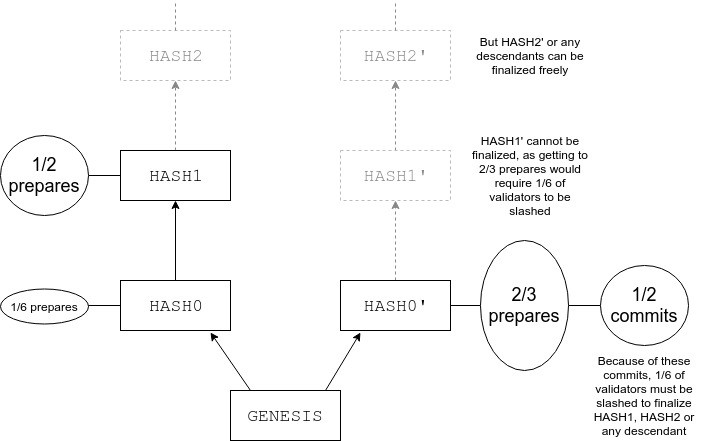
\includegraphics[width=400px]{fork_choice_rule.jpeg}

In this case, $HASH1$ or any descendant thereof cannot be finalized without slashing $\frac{1}{6}$ of validators. However, miners on a proof of work chain would interpret $HASH1$ as the head and forever keep mining descendants of it, ignoring the chain based on $HASH0'$ which actually could get finalized.

In fact, when \textit{any} checkpoint gets $k > \frac{1}{3}$ commits, no conflicting checkpoint can get finalized without $k - \frac{1}{3}$ of validators getting slashed. This necessitates modifying the fork choice rule used by participants in the underlying proposal mechanism (as well as users and validators): instead of blindly following a longest-chain rule, there needs to be an overriding rule that (i) finalized checkpoints are favored, and (ii) when there are no further finalized checkpoints, checkpoints with more (justified) commits are favored.

One complete description of such a rule would be:

\begin{enumerate}
\item Start with HEAD equal to the genesis of the chain.
\item Select the descendant checkpoint of HEAD with the most commits (only justified checkpoints are admissible)
\item Repeat (2) until no descendant with commits exists.
\item Choose the longest proof of work chain from there.
\end{enumerate}

The commit-following part of this rule can be viewed in some ways as mirroring the "greegy heaviest observed subtree" (GHOST) rule that has been proposed for proof of work chains [cite]. The symmetry is as follows. In GHOST, a node starts with the head at the genesis, then begins to move forward down the chain, and if it encounters a block with multiple children then it chooses the child that has the larger quantity of work built on top of it (including the child block itself and its descendants).

In this algorithm, we follow a similar approach, except we repeatedly seek the child that comes the closest to achieving finality. Commits on a descendant are implicitly commits on all of its ancestors, and so if a given descendant of a given block has more commits than any other descendant, then we know that all children along the chain from the head to this descendant are closer to finality than any of their siblings; hence, looking for the \textit{descendant} with the most commits and not just the \textit{child} replicates the GHOST principle most faithfully. Finalizing a checkpoint requires $\frac{2}{3}$ commits within a \textit{single} epoch, and so we do not try to sum up commits across epochs and instead simply take the maximum.

This rule ensures that if there is a checkpoint such that no conflicting checkpoint can be finalized without at least some validators violating slashing conditions, then this is the checkpoint that will be viewed as the ``head'' and thus that validators will try to commit on.

\section{Dynamic Validator Sets}

In an open protocol, the validator set needs to be able to change; old validators need to be able to withdraw, and new validators need to be able to enter. To accomplish this end, we define a variable kept track of in the state called the \textit{dynasty} counter. When a user sends a ``deposit'' transaction to become a validator, if this transaction is included in dynasty $n$, then the validator will be \textit{inducted} in dynasty $n+2$. The dynasty counter is incremented when the chain detects that the checkpoint of the current epoch that is part of its own history has been finalized (that is, the checkpoint of epoch $e$ must be finalized during epoch $e$, and the chain must learn about this before epoch $e$ ends). In simpler terms, when a user sends a ``deposit'' transaction, they need to wait for the transaction to be finalized, and then they need to wait again for that epoch to be finalized; after this, they become part of the validator set. We call such a validator's \textit{start dynasty} $n+2$.

For a validator to leave, they must send a ``withdraw'' message. If their withdraw message gets included during dynasty $n$, the validator similarly leaves the validator set during dynasty $n+2$; we call $n+2$ their \textit{end dynasty}. When a validator withdraws, their deposit is locked for four months before they can take their money out; if they are caught violating a slashing condition within that time then their deposit is forfeited.

For a checkpoint to be justified, it must be prepared by a set of validators which contains (i) at least $\frac{2}{3}$ of the current dynasty (that is, validators with $startDynasty \le curDynasty < endDynasty$), and (ii) at least $\frac{2}{3}$ of the previous dynasty (that is, validators with $startDynasty \le curDynasty - 1 < endDynasty$. Finalization with commits works similarly. The current and previous dynasties will usually mostly overlap; but in cases where they substantially diverge this ``stitching'' mechanism ensures that dynasty divergences do not lead to situations where a finality reversion or other failure can happen because different messages are signed by different validator sets and so equivocation is avoided.

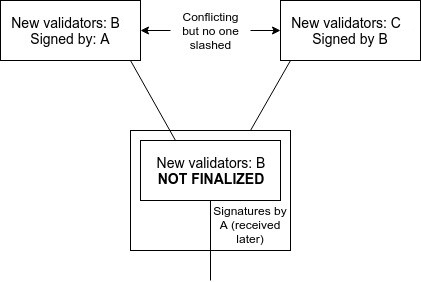
\includegraphics[width=250px]{validator_set_misalignment.png}

\section{Mass Crash Failure Recovery}

Suppose that more than one third of validators crash-fail at the same time; that is, they either are no longer connected to the network due to a network partition, or their computers fail, or they do this as a malicious attack. Then, no checkpoint will be able to get finalized.

We can recover from this by instituting a rule that validators who do not prepare or commit for a long time start to see their deposit sizes decrease (depending on the desired economic incentives this can be either a compulsory partial withdrawal or an outright confiscation), until eventually their deposit sizes decrease low enough that the validators that \textit{are} preparing and committing are once again a $\frac{2}{3}$ supermajority.

Note that this does introduce the possibility of two conflicting checkpoints being finalized, with validators only losing money on one of the two checkpoints:

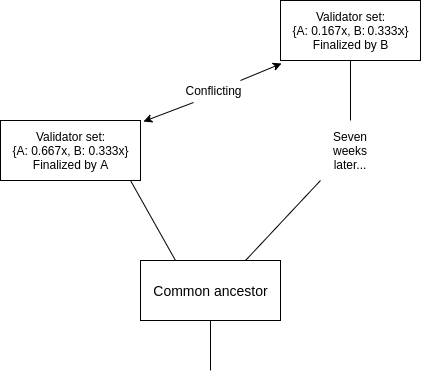
\includegraphics[width=300px]{CommitsSync.png}

If the goal is simply to achieve maximally close to 50\% fault tolerance, then clients should simply favor the finalized checkpoint that they received earlier. However, if clients are also interested in defeating 51\% censorship attacks, then they may want to at least sometimes choose the minority chain. All forms of ``51\% attacks'' can thus be resolved fairly cleanly via ``user-activated soft forks'' that reject what would normally be the dominant chain. Particularly, note that finalizing even one block on the dominant chain precludes the attacking validators from preparing on the minority chain because of \textbf{PREPARE\_COMMIT\_CONSISTENCY}, at least until their balances decrease to the point where the minority can commit, so such a fork would also serve the function of costing the majority attacker a very large portion of their deposits.

\section{Conclusions}

This introduces the basic workings of Casper the Friendly Finality Gadget's prepare and commit mechanism and fork choice rule, in the context of Byzantine fault tolerance analysis. Separate papers will serve the role of explaining and analyzing incentives inside of Casper, and the different ways that they can be parametrized and the consequences of these paramtrizations.

\section{References}
\bibliographystyle{abbrv}
\bibliography{main}
\begin{itemize}
\item Aviv Zohar and Yonatan Sompolinsky, ``Fast Money Grows on Trees, not Chains'': https://eprint.iacr.org/2013/881.pdf
\item Jae Kwon, ``Tendermint'': http://tendermint.org/tendermint.pdf
\item Miguel Castro and Barbara Liskov, ``Practical Byzantine Fault Tolerance'': http://pmg.csail.mit.edu/papers/osdi99.pdf 
\end{itemize}

\end{document}
